\chapter{文本处理}
\label{chap:processing_words}

\marginpar{111}
本章的程序指向一个共同主题: 文本处理. 示例程序涵盖的范围包括随机单词
与句子的生成 (生成的句子可以和用户进行有限的对话), 以及文本处理. 大多数示例
程序都很简单, 它们只是起说明作用, 但是, 其中一些文档准备程序的确拥有实际
用途.

\section{随机文本发生器}
\label{sec:random_text_generation}

生成随机数据的程序有许多种用途. 这种程序可以用内建函数 \texttt{rand} 来
创建, 该函数每次被调用时, 都会返回一个伪随机数. \texttt{rand} 每次都使用
同一个种子数来生成随机数, 所以, 如果你想要得到一个不同的随机数序列, 你
就必须调用一次 \texttt{srand()}, 它根据当前时间计算出一个种子数, 并用
该种子数初始化 \texttt{rand}.

\subsection{随机选择}
\label{subsec:random_choices}

\texttt{rand} 每次被调用时都会返回 一个大于等于 0, 小于 1 的浮点数, 但是
一般来说, 更通常的需求是返回一个 \texttt{1} 到 \texttt{n} 之间的随机整数,
我们可以用 \texttt{rand} 来实现:
\begin{awkcode}
    # randint - return random integer x, 1 <= x <= n

    function randint(n) {
        return int(n * rand()) + 1
    }
\end{awkcode}
\texttt{randint(n)} 按比例调整 \texttt{rand} 的返回值, 调整后的值大于
等于 \texttt{0} 并且小于 \texttt{n}, 将小数部分截去可以得到 \texttt{0} 
到 \texttt{n-1} 的整数, 然后再加 1, 就是 \texttt{1} 到 \texttt{n} 之间的 
整数.

我们可以用 \texttt{randint} 来随机选择一个字母:
\marginpar{112}
\begin{awkcode}
    # randlet - generate random lower-case letter

    function randlet() {
        return substr("abcdefghijklmnopqrstuvwxyz", randint(26), 1)
    }
\end{awkcode}

利用 \texttt{randint}, 很容易就可以从一个 \texttt{n} 项的数组中随机选择一
个元素:
\begin{awkcode}
    print x[randint(n)]
\end{awkcode}
一个更有趣的问题是从某个数组中随机选择几项, 被选中的项必须按照原来的顺序
排列. 举例来说, 如果数组 \texttt{x} 按照升序排列, 则被选中的元素也要按照
升序排列.

函数 \texttt{choose} 从数组 \texttt{A} 的前 \texttt{n} 中随机选择
\texttt{k} 个元素, 并按照原来的顺序打印出来:
\begin{awkcode}
    # choose - print in order k random elements from A[1]..A[n]

    function choose(A, k, n,    i) {
        for (i = 1; n > 0; i++)
            if (rand() < k/n--) {
                print A[i]
                k--
            }
    }
\end{awkcode}
在函数内, \texttt{k} 是还需要打印的项的数目, \texttt{n} 是数组中等待检验
的元素个数. 打印第 \texttt{i} 个元素的条件是 \verb'rand() < k/n', 每当有
一个元素被打印出来, \texttt{k} 就递减一次, 每当判断条件 \verb'rand() < k/n'
被测试一次, \texttt{n} 就递减一次.

\begin{exercise}
    测试 \texttt{rand} 的输出是不是真的随机数.
\end{exercise}
\begin{exercise}
    写一个程序, 该程序生成 1 到 $n$ 之间的 $k$ 个不同的随机整数,
    程序的时间复杂 度与 $k$ 成正比.
\end{exercise}
\begin{exercise}
    写一个程序, 该程序生成随机的桥牌手 (bridge hands).
\end{exercise}

\subsection{废话生成器}
\label{subsec:cliche_generation}

我们的下一个例子是废话生成器 (cliche generator),
它根据已有的废话重新创建一个新的出来. 输入是一个句子集合:
\begin{file}
    A rolling stone:gathers no moss.
    History:repeats itself.
    He who lives by the sword:shall die by the sword.
    A jack of all trades:is master of none.
    Nature:abhors a vacuum.
    Every man:has a price.
    All's well that:ends well.
\end{file}
冒号将主语和谓语分开. 我们的废话生成器随机选择一个主语与另一个谓语作组合,
\marginpar{113}
如果运气好的话, 可能会产生很有意思的格言警句:
\begin{file}
    A rolling stone repeats itself.
    History abhors a vacuum.
    nature repeats itself.
    All's well that gathers no moss.
    He who lives by the sword has a price.
\end{file}
程序的代码实现非常明确:
\begin{awkcode}
    # cliche - generate an endless stream of cliches
    #     input:  lines of form subject:predicate
    #     output: lines of random subject and random predicate

    BEGIN { FS = ":" }
          { x[NR] = $1; y[NR] = $2 }
    END   { for (;;) print x[randint(NR)], y[randint(NR)] }

    function randint(n) { return int(n * rand()) + 1 }
\end{awkcode}
请注意, 程序中的死循环是有意为之.

\subsection{随机语句}
\label{subsec:random_sentences}

\cterm{上下文无关语法} (\term{contex-free grammar}) 指的是一组规则, 这组
规则定义了如何生成或分析一个语句集合. 每一条规则 (称为 \cterm{产生式}
(\term{production})) 都具有形式:
\begin{pattern}
    \indent\indent\textit{A} $\longrightarrow$ \textit{B C D} ...
\end{pattern}
该产生式的意思是每一个 \textit{A} 都可以被 ``重写'' 为 \textit{B C D ...}.
产生式左边的符号 (\textit{A}) 称为 \cterm{非终结符} (\term{nonterminal}),
它可以被进一步地扩展. 产生式右边的符号可以是非终结符 (可以是多个
\textit{A}) 或 \cterm{终结符} (\term{terminal}), 终结符指的是不能被扩展的
符号. 多个产生式可以共享同一个非终结符, 终结符与非终结符也可以在产生式的
右边出现多次.

我们将在第 \ref{chap:little_languages} 章展示 awk 的部分语法规则, 并利用
该规则开发一个语法分析器, 用来分析 awk 程序. 然而在这一章, 我们感兴趣的是
规则的生成, 而不是分析. 举例来说, 类似 ``the boy walks slowly'' 和 ``the
girl runs very very quickly'' 这样的句子可以用下面的语法来描述:
\begin{file}
    Sentence -> Nounphrase Verbphrase
    Nounphrase -> the boy
    Nounphrase -> the girl
    Verbphrase -> Verb Modlist Adverb
    Verb -> runs
    Verb -> walks
    Modlist -> very Modlist
    Adverb -> quickly
    Adverb -> slowly
\end{file}

\marginpar{114}
如下所示, 产生式为非终结符生成语句. 假设 \texttt{Sentence} 是起始非终结符,
那么选择一条以该符号作为左部的产生式:
\begin{file}
    Sentence -> Nounphrase Verbphrase
\end{file}
接下来, 从右部选择一个非终结符, 比如说 \texttt{Nounphrase}, 然后用以
\texttt{Nounphrase} 作为左部的产生式替换掉 \texttt{Nounphrase}:
\begin{file}
    Sentence -> Nounphrase Verbphrase
             -> the boy Verbphrase
\end{file}
不断地使用该方法, 直到所有的非终结符都被替换掉为止:
\begin{file}
    Sentence -> Nounphrase Verbphrase
             -> the boy Verbphrase
             -> the bov Verb Modlist Adverb
             -> the boy walks very Modlist Adverb
             -> the boy walks very Adverb
             -> the boy walks very quickly
\end{file}
\texttt{Sentence} 的最终展开结果是一个句子. 非终结符的推导过程与我们在初
级学校所学到的语句图 (sentence-diagram) 刚好相反: 我们现在是把动词短语拆
分成动词与副词, 而不是把动词与副词组合成动词短语.

\texttt{Modlist} 的产生式比较有趣. 一条规则是说用 \texttt{very Modlist}
替换 \texttt{Modlist}, 每次使用这条规则都会使句子变长. 幸运地是, 只要运用
另一条产生式规则 (该规则用空字符串替换掉 \texttt{Modlist}) 就可以终止潜在
的无限循环.

我们现在要开发一个程序, 该程序根据语法生成语句, 每次生成都从一个指定的非
终结符开始. 程序从文件中读取语法规则, 记录下每一个左部出现的次数, 
左部所拥有的右部的个数, 以及它们各自的组成成分. 然后, 每输入一个非
终结符, 就会为该非终结符生成一个随机语句.

程序使用三个数组来存放语法规则:
\texttt{lhs[A]} 给出了非终结符 \texttt{A} 的产 
生式个数, \texttt{rhscnt[A, i]} 存放的是 \texttt{A} 的第 \texttt{i} 条产生
式右部的符号个数, \texttt{rhslist[A, i, j]} 存放的是 \texttt{A} 的第 
\texttt{i} 条产生式右部的第 \texttt{j} 个符号. 对于前面提到的语法规则, 
三个数组的内容分别是:

\begin{tabular}{ccc}

\begin{varwidth}[t]{\textwidth}
\vspace{0pt}
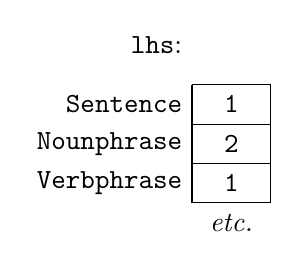
\begin{tikzpicture}
    \pgfmathsetmacro\height{0.5};
    \pgfmathsetmacro\maxheight{4.5};

    \foreach \i in {0,...,3}
        \draw (0, \maxheight - \i * \height) -- (1, \maxheight - \i *
        \height);
    \draw (0, \maxheight - 0) -- (0, \maxheight - 3 * \height);
    \draw (1, \maxheight - 0) -- (1, \maxheight - 3 * \height);
    \node[left] at (0, \maxheight - \height * 0.5) {\texttt{Sentence}};
    \node[left] at (0, \maxheight - \height * 1.5) {\texttt{Nounphrase}};
    \node[left] at (0, \maxheight - \height * 2.5) {\texttt{Verbphrase}};
    \node at (0.5, \maxheight - \height * 0.5) {\texttt{1}};
    \node at (0.5, \maxheight - \height * 1.5) {\texttt{2}};
    \node at (0.5, \maxheight - \height * 2.5) {\texttt{1}};
    \node at (0.5, \maxheight - \height * 3.5) {\textit{etc.}};
    \node[left] at (0, \maxheight + 0.5) {\texttt{lhs}:};
\end{tikzpicture}
\end{varwidth}
&
\begin{varwidth}[t]{\textwidth}
\vspace{0pt}
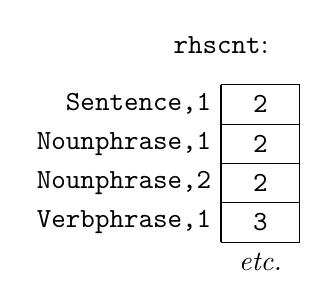
\begin{tikzpicture}
    \pgfmathsetmacro\height{0.5};
    \pgfmathsetmacro\maxheight{4.5};

    \foreach \i in {0,...,4}
        \draw (0, \maxheight - \i * \height) -- (1, \maxheight - \i *
        \height);
    \draw (0, \maxheight - 0) -- (0, \maxheight - 4 * \height);
    \draw (1, \maxheight - 0) -- (1, \maxheight - 4 * \height);
    \node[left] at (0, \maxheight - \height * 0.5) {\texttt{Sentence,1}};
    \node[left] at (0, \maxheight - \height * 1.5) {\texttt{Nounphrase,1}};
    \node[left] at (0, \maxheight - \height * 2.5) {\texttt{Nounphrase,2}};
    \node[left] at (0, \maxheight - \height * 3.5) {\texttt{Verbphrase,1}};
    \node at (0.5, \maxheight - \height * 0.5) {\texttt{2}};
    \node at (0.5, \maxheight - \height * 1.5) {\texttt{2}};
    \node at (0.5, \maxheight - \height * 2.5) {\texttt{2}};
    \node at (0.5, \maxheight - \height * 3.5) {\texttt{3}};
    \node at (0.5, \maxheight - \height * 4.5) {\textit{etc.}};
    \node at (0, \maxheight + 0.5) {\texttt{rhscnt}:};
\end{tikzpicture}
\end{varwidth}
&
\begin{varwidth}[t]{\textwidth}
\vspace{0pt}
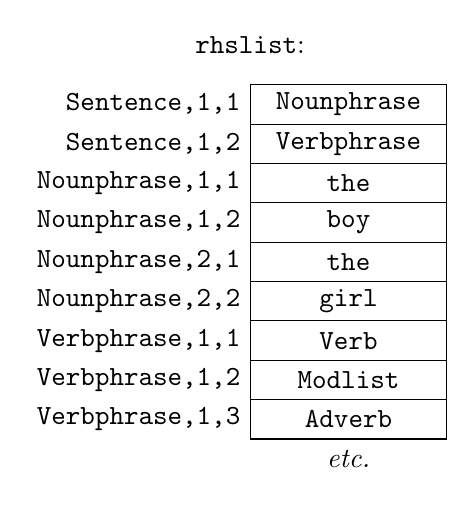
\begin{tikzpicture}
    \pgfmathsetmacro\height{0.5};
    \pgfmathsetmacro\maxheight{4.5};

    \foreach \i in {0,...,9}
        \draw (0, \maxheight - \i * \height) -- (2.5, \maxheight - \i *
        \height);
    \draw (0, \maxheight - 0) -- (0, \maxheight - 9 * \height);
    \draw (2.5, \maxheight - 0) -- (2.5, \maxheight - 9 * \height);
    \node[left] at (0, \maxheight - \height * 0.5) {\texttt{Sentence,1,1}};
    \node[left] at (0, \maxheight - \height * 1.5) {\texttt{Sentence,1,2}};
    \node[left] at (0, \maxheight - \height * 2.5) {\texttt{Nounphrase,1,1}};
    \node[left] at (0, \maxheight - \height * 3.5) {\texttt{Nounphrase,1,2}};
    \node[left] at (0, \maxheight - \height * 4.5) {\texttt{Nounphrase,2,1}};
    \node[left] at (0, \maxheight - \height * 5.5) {\texttt{Nounphrase,2,2}};
    \node[left] at (0, \maxheight - \height * 6.5) {\texttt{Verbphrase,1,1}};
    \node[left] at (0, \maxheight - \height * 7.5) {\texttt{Verbphrase,1,2}};
    \node[left] at (0, \maxheight - \height * 8.5) {\texttt{Verbphrase,1,3}};
    \node at (1.25, \maxheight - \height * 0.5) {\texttt{Nounphrase}};
    \node at (1.25, \maxheight - \height * 1.5) {\texttt{Verbphrase}};
    \node at (1.25, \maxheight - \height * 2.5) {\texttt{the}};
    \node at (1.25, \maxheight - \height * 3.5) {\texttt{boy}};
    \node at (1.25, \maxheight - \height * 4.5) {\texttt{the}};
    \node at (1.25, \maxheight - \height * 5.5) {\texttt{girl}};
    \node at (1.25, \maxheight - \height * 6.5) {\texttt{Verb}};
    \node at (1.25, \maxheight - \height * 7.5) {\texttt{Modlist}};
    \node at (1.25, \maxheight - \height * 8.5) {\texttt{Adverb}};
    \node at (1.25, \maxheight - \height * 9.5) {\textit{etc.}};
    \node at (0, \maxheight + 0.5) {\texttt{rhslist}:};
\end{tikzpicture}
\end{varwidth}
\end{tabular}

\marginpar{115}
程序的源代码是:
\begin{awkcode}
    # sentgen - random sentence generator
    #   input:  grammar file; sequence of nonterminals
    #   output: a random sentence for each nonterminal

    BEGIN {  # read rules from grammar file
        while (getline < "grammar" > 0)
            if ($2 == "->") {
                i = ++lhs[$1]              # count lhs
                rhscnt[$1, i] = NF-2       # how many in rhs
                for (j = 3; j <= NF; j++)  # record them
                   rhslist[$1, i, j-2] = $j
            } else
                print "illegal production: " $0
    }

    {   if ($1 in lhs) {  # nonterminal to expand
            gen($1)
            printf("\n")
        } else 
            print "unknown nonterminal: " $0   
    }

    function gen(sym,    i, j) {
        if (sym in lhs) {       # a nonterminal
            i = int(lhs[sym] * rand()) + 1   # random production
            for (j = 1; j <= rhscnt[sym, i]; j++) # expand rhs's
                gen(rhslist[sym, i, j])
        } else
            printf("%s ", sym)
    }
\end{awkcode}

函数 \texttt{gen("A")} 为非终结符 \texttt{A} 生成一条语句. 如果前一次的扩展
引入了非终结符, 那么函数通过递归调用自身来展开. 请记住, 所有被递归函数用%
\marginpar{116}%
到的临时变量都需要出现在函数的参数列表中, 如果某个变量没有出现在参数列表,
那它就是全局变量, 此时程序就无法正确地工作.

我们把右部个数及其组成成分分别存放在两个数组中, 不过实际上, 不使用下标
来编码不同的字段也是有可能的, 在其他语言中可以通过记录或结构体来实现. 
举例来说, 数组 \texttt{rhscnt[i,j]} 可以是 \texttt{rhslist} 的元素,
表示成 \texttt{rhslist[i,j,"cnt"]}.\footnote{原文为 We chose to use
    separate arrays for the right-hand-side counts and components, but it
    is possible instead to use subscripts to encode different fields,
    rather like records or structures in other languages. For example, the
    array \texttt{rhscnt[i,j]} could be part of \texttt{rhslist}, as
    \texttt{rhslist[i,j,"cnt"]}.}

\begin{exercise}
    写一套语法规则, 该规则能够生成关于某学科的, 听起来貌似合理的文本 ---
    商业, 政治, 计算科学都是很好的选择.\footnote{原文为 Write a grammar for
        generating plausible-sounding text from a field that appeals to you
    -- business, politics, and computing are all good possibilities.}
\end{exercise}

\begin{exercise}
    在某些语法规则下, 语句生成程序很有可能落入到这样一种境地:
    推导过程越来越长, 却没有停下来的迹象, 添加一条机制, 使得程序可以限制
    推导过程的长度.
\end{exercise}

\begin{exercise}
    给语法规则加上权重, 使得对同一个非终结符来说, 它的各个展开规则被选中
    的概率是不同的.
\end{exercise}

\begin{exercise}
    实现一个非递归的语句生成程序.
\end{exercise}

\section{交互式的文本处理}
\label{sec:interactive_text_manipulation}

使用 awk 很容易就可以写出一个交互式程序, 我们将通过两个示例程序来阐明
基本思路. 第一个程序测试运算能力, 第二个程序测试某一特定领域的相关知识.

\subsection{技巧测试: 运算}
\label{subsec:skills_testing_arithmetic}

下面的程序 \texttt{arith} (最适用于幼儿) 显示一系列加法运算问题, 比如 
\begin{file}
    7 + 9 = ?
\end{file}
在每个问题之后, 用户输入问题的答案. 如果回答是正确的, 用户就会收到一句
赞美, 然后显示下一个问题; 如果回答是错误的, 那么程序会再次请求输入答案;
如果用户没有输入答案, 那么在显示下一个问题之前, 程序输出正确答案.

调用程序的命令行有两种形式:
\begin{pattern}
    \indent\texttt{awk -f arith} \par 
    \indent\texttt{awk -f arith} \textit{n}
\end{pattern}
如果在 \texttt{arith} 之后有一个参数, 程序将使用该参数限制每个问题的数的
最大值. 该参数被读取之后, \texttt{ARGV[1]} 被设置为 \texttt{"-"},
于是程序从标准输入读取用户的回答. 如果没有指定参数, 那么数的最大值就是
10.
\marginpar{117}
\begin{awkcode}
    # arith - addition drill
    #   usage:  awk -f arith [ optional problem size ]
    #   output: queries of the form "i + j = ?"

    BEGIN {
        maxnum = ARGC > 1 ? ARGV[1] : 10   # default size is 10
        ARGV[1] = "-"  # read standard input subsequently
        srand()        # reset rand from time of day
        do {
            n1 = randint(maxnum)
            n2 = randint(maxnum)
            printf("%g + %g = ? ", n1, n2)
            while ((input = getline) > 0)
                if ($0 == n1 + n2) {
                    print "Right!"
                    break
                } else if ($0 == "") {
                    print n1 + n2
                    break
                } else
                    printf("wrong, try again: ")
        } while (input > 0)
    }

    function randint(n) { return int(rand()*n)+1 }
\end{awkcode}
